\chapter{Experimentações}

Esta seção apresenta o protótipo desenvolvido para a parte web da solução. Serão mostradas as telas de interação com o aluno e professor. Para tanto, foi definida uma metodologia~\ref{section:metodologia-testes} das experimentações que explicará como foi dividido os cenários de testes.
A seção~\ref{section:interface-aluno} mostra o fluxo de execução desde o primeiro acesso do aluno à visualização do seu estilo de aprendizagem. A seção~\ref{section:interface-docente} mostra o fluxo de execução do docente que deseja verificar o estilo de aprendizagem de seus alunos.

Por fim, o capítulo de resultados~\ref{section:resultados} destaca todos os resultados esperados do cenários do aluno e dos objetivos do projeto.

\section{Metodologia de Testes}\label{section:metodologia-testes}

A metodologia de testes foi dividida em dois cenários. O primeiro deles é o cenário onde o aluno faz o primeiro acesso ao sistema e deseja conhecer o seu estilo de aprendizagem. É seguido então um fluxo de execução para que este aluno possa realizar o questionário de estilos de aprendizagem. No fim do fluxo, espera-se que o aluno saiba o seu estilo de aprendizagem.

O segundo cenário aborda o acesso do docente ao sistema, desejando saber o estilo de aprendizagem dos alunos de sua turma. É demonstrado um fluxo de execução para que ele autentique-se no sistema e acesse os dados de sua turma. Ao final deste fluxo, é esperado que o docente saiba o estilo de aprendizagem de todos os alunos que realizaram o questionário.
As duas próximas seções mostram os fluxos explicados.

\section{Demonstração da Interface com Aluno}\label{section:interface-aluno}
O fluxo inicia-se quando o aluno acessa a interface principal do Sistema~\ref{fig:frank-tela-aluno-inicial}, mostrando uma tela de boas vindas. O usuário seleciona vai para a tela de autenticação e o Sistema exige o login e a senha de acesso~\ref{fig:frank-tela-aluno-login}. Caso o usuário informe o login inválido o Sistema apresenta a tela de erro~\ref{fig:frank-tela-login-invalido}, solicitando novamente os dados para autenticação.

\begin{figure}
	\centering
	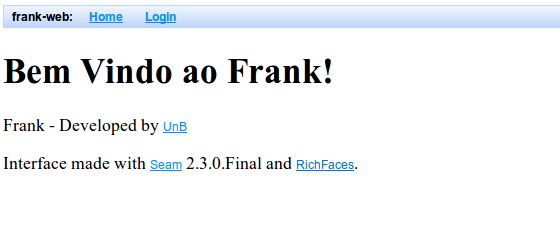
\includegraphics[scale=0.6]{images/frank-tela-aluno-inicial.png}
	\caption{Tela Inicial do Sistema.}
	\label{fig:frank-tela-aluno-inicial}
\end{figure}


\begin{figure}
	\centering
	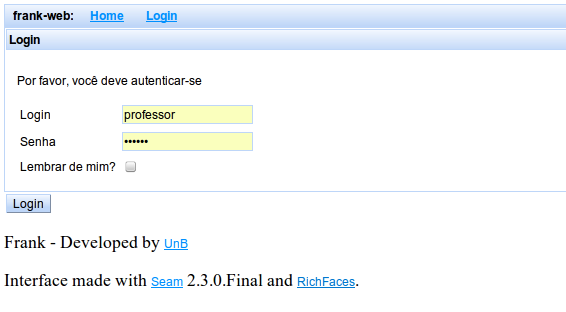
\includegraphics[scale=0.6]{images/frank-tela-aluno-login.png}
	\caption{Tela de Autenticação do Sistema.}
	\label{fig:frank-tela-aluno-login}
\end{figure}

\begin{figure}
	\centering
	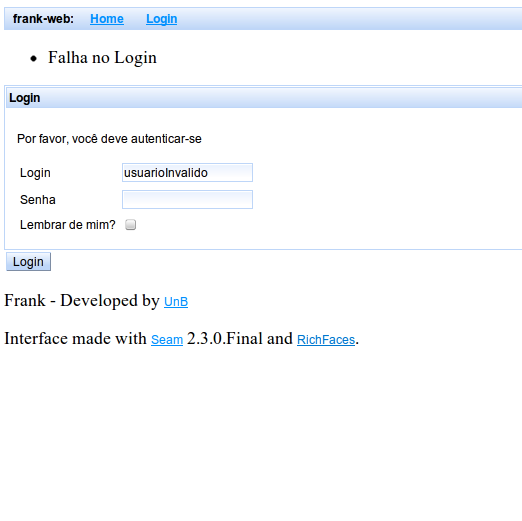
\includegraphics[scale=0.6]{images/frank-tela-login-invalido.png}
	\caption{Tela de Erro de Autenticação do Sistema.}
	\label{fig:frank-tela-login-invalido}
\end{figure}

Após a autenticação, o usuário com perfil de aluno realiza o primeiro acesso ao Sistema. Ele detecta que o usuário não fez o questionário de estilos de aprendizagem e apresenta a tela de convite ao preenchimento do mesmo~\ref{fig:frank-tela-aluno-prim-acesso}.

\begin{figure}
	\centering
	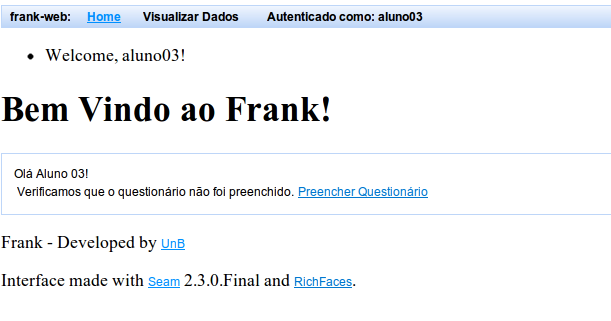
\includegraphics[scale=0.6]{images/frank-tela-aluno-prim-acesso.png}
	\caption{Tela de convite ao preenchimento do questionário de estilos de aprendizagem.}
	\label{fig:frank-tela-aluno-prim-acesso}
\end{figure}

O usuário então entra na tela de preenchimento do questionário~\ref{fig:frank-tela-aluno-preencher-questionario}, preenche todas as respostas de acordo com suas características e em seguida seleciona o botão "Confirmar". O Sistema envia os dados para o SMA e o seu estilo de aprendizado é inferido.

\begin{figure}
	\centering
	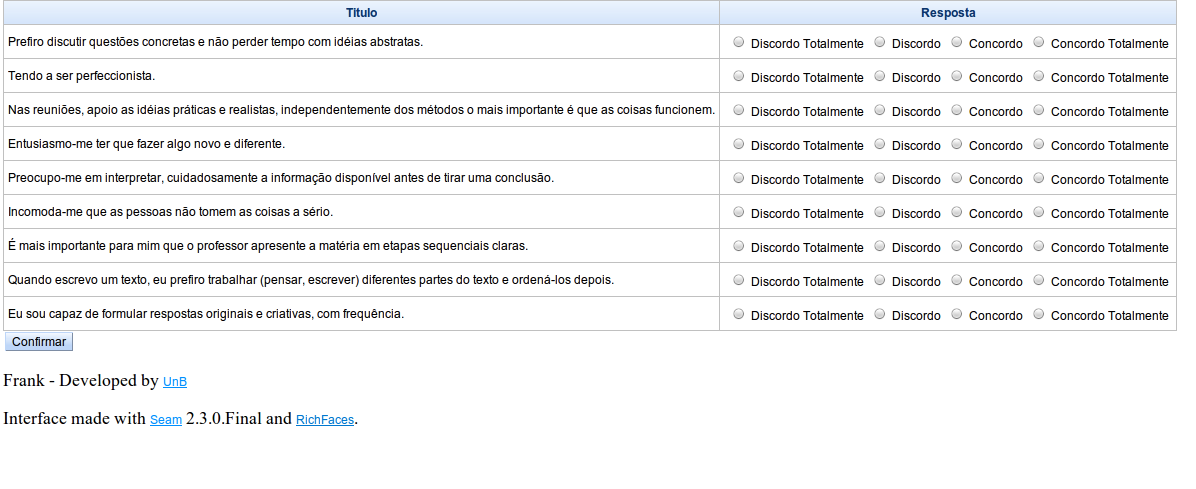
\includegraphics[scale=0.48]{images/frank-tela-aluno-preencher-questionario.png}
	\caption{Tela de prenchimento do questionário.}
	\label{fig:frank-tela-aluno-preencher-questionario}
\end{figure}

Por fim, o Sistema exibe o resultado final do processamento do SMA na tela de boas vindas~\ref{fig:frank-tela-aluno-inferencia-estilo}. Dessa forma, o usuário verá sempre o seu estilo de aprendizagem atualizado ao acessar o Sistema.

\begin{figure}
	\centering
	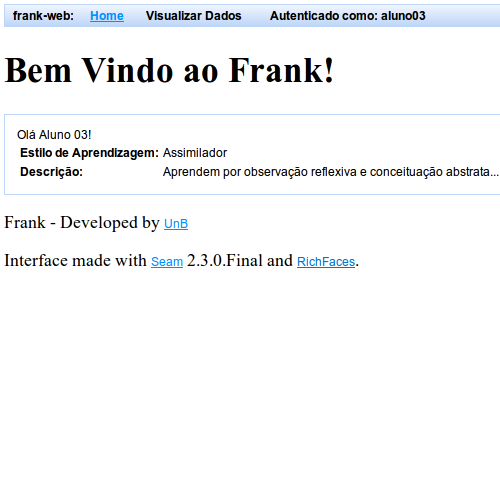
\includegraphics[scale=0.48]{images/frank-tela-aluno-inferencia-estilo.png}
	\caption{Tela de visualização do estilo de aprendizagem inferido.}
	\label{fig:frank-tela-aluno-inferencia-estilo}
\end{figure}

\section{Demonstração da Interface com Docente}\label{section:interface-docente}
O fluxo do docente é semelhante ao fluxo do aluno até a autenticação passo de autenticação~\ref{fig:frank-tela-aluno-login}. O Sistema distingue os usuários neste momento e, no caso do Docente, renderiza uma tela diferente devido ao seu perfil. Ele renderiza a tela de visualização de turmas às quais pertencem ao docente em questão.

\begin{figure}
	\centering
	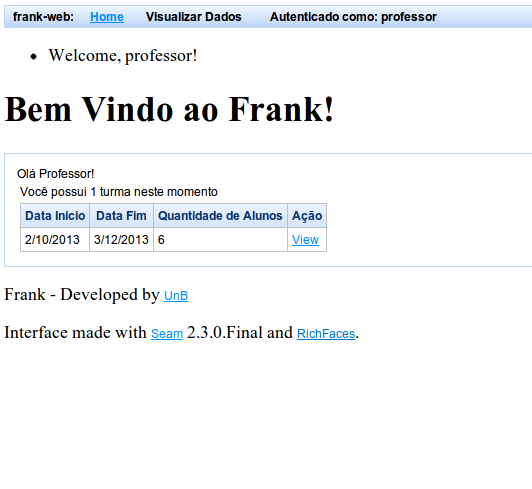
\includegraphics[scale=0.48]{images/frank-tela-professor-acesso.png}
	\caption{Tela inicial do usuário com o perfil de docente.}
	\label{fig:frank-tela-professor-acesso}
\end{figure}

O Docente seleciona a turma desejada e o Sistema aprensenta a tela de visualização de estilos de aprendizagem dos alunos pertencentes àquela turma. É importante notar que nem todos os alunos possuem um estilo de aprendizagem inferido visto que, estes devem fazer acesso ao Sistema para a inferência do estilo ou, no futuro, podem possuir desvios no seu estilo de aprendizagem.

\begin{figure}
	\centering
	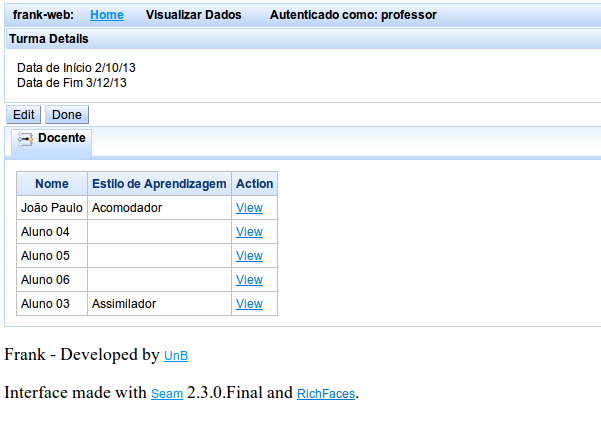
\includegraphics[scale=0.48]{images/frank-tela-professor-visualizar-turma.png}
	\caption{Tela de visualização do estilo de aprendizagem por turma.}
	\label{fig:frank-tela-professor-visualizar-turma}
\end{figure}

\section{Resultados}\label{section:resultados}
Após a execução das experimentações, foi possível observar vários aspectos do sistema. O primeiro deles é a assistência do aluno por meio do grupo de trabalho específico para ele, com os agentes cognitivo, metacognitivo e afetivo. Com esse grupo de trabalho será possível a inferência do seu modelo multidimensional por meio de dados de Ambientes Virtuais de Aprendizagem.

Além disso, por meio de preenchimento de questionário e consequentemente a modelagem explícita, houve a determinação do seu estilo de aprendizagem. O agente cognitivo possui inteligência para interpretar as respostas do questionário e determinar o seu estilo de aprendizagem.

Por fim, através do cenário do docente, foi possível visualizar a notificação do estilo de aprendizagem dos seus alunos feito pela plataforma.
